
%% LyX 2.2.1 created this file.  For more info, see http://www.lyx.org/.
%% Do not edit unless you really know what you are doing.
\documentclass[12pt]{beamer}\usepackage[]{graphicx}\usepackage[]{color}
%% maxwidth is the original width if it is less than linewidth
%% otherwise use linewidth (to make sure the graphics do not exceed the margin)
\makeatletter
\def\maxwidth{ %
  \ifdim\Gin@nat@width>\linewidth
    \linewidth
  \else
    \Gin@nat@width
  \fi
}
\makeatother

\definecolor{fgcolor}{rgb}{0.345, 0.345, 0.345}
\newcommand{\hlnum}[1]{\textcolor[rgb]{0.686,0.059,0.569}{#1}}%
\newcommand{\hlstr}[1]{\textcolor[rgb]{0.192,0.494,0.8}{#1}}%
\newcommand{\hlcom}[1]{\textcolor[rgb]{0.678,0.584,0.686}{\textit{#1}}}%
\newcommand{\hlopt}[1]{\textcolor[rgb]{0,0,0}{#1}}%
\newcommand{\hlstd}[1]{\textcolor[rgb]{0.345,0.345,0.345}{#1}}%
\newcommand{\hlkwa}[1]{\textcolor[rgb]{0.161,0.373,0.58}{\textbf{#1}}}%
\newcommand{\hlkwb}[1]{\textcolor[rgb]{0.69,0.353,0.396}{#1}}%
\newcommand{\hlkwc}[1]{\textcolor[rgb]{0.333,0.667,0.333}{#1}}%
\newcommand{\hlkwd}[1]{\textcolor[rgb]{0.737,0.353,0.396}{\textbf{#1}}}%
\let\hlipl\hlkwb

\usepackage{framed}
\makeatletter
\newenvironment{kframe}{%
 \def\at@end@of@kframe{}%
 \ifinner\ifhmode%
  \def\at@end@of@kframe{\end{minipage}}%
  \begin{minipage}{\columnwidth}%
 \fi\fi%
 \def\FrameCommand##1{\hskip\@totalleftmargin \hskip-\fboxsep
 \colorbox{shadecolor}{##1}\hskip-\fboxsep
     % There is no \\@totalrightmargin, so:
     \hskip-\linewidth \hskip-\@totalleftmargin \hskip\columnwidth}%
 \MakeFramed {\advance\hsize-\width
   \@totalleftmargin\z@ \linewidth\hsize
   \@setminipage}}%
 {\par\unskip\endMakeFramed%
 \at@end@of@kframe}
\makeatother

\definecolor{shadecolor}{rgb}{.97, .97, .97}
\definecolor{messagecolor}{rgb}{0, 0, 0}
\definecolor{warningcolor}{rgb}{1, 0, 1}
\definecolor{errorcolor}{rgb}{1, 0, 0}
\newenvironment{knitrout}{}{} % an empty environment to be redefined in TeX

\usepackage{alltt}
\usepackage[T1]{fontenc}
\usepackage[utf8]{inputenc}
\setcounter{secnumdepth}{3}
\setcounter{tocdepth}{3}
\usepackage{url}
\ifx\hypersetup\undefined
  \AtBeginDocument{%
    \hypersetup{unicode=true,pdfusetitle,
 bookmarks=true,bookmarksnumbered=false,bookmarksopen=false,
 breaklinks=false,pdfborder={0 0 0},pdfborderstyle={},backref=false,colorlinks=false}
  }
\else
  \hypersetup{unicode=true,pdfusetitle,
 bookmarks=true,bookmarksnumbered=false,bookmarksopen=false,
 breaklinks=false,pdfborder={0 0 0},pdfborderstyle={},backref=false,colorlinks=false}
\fi
\usepackage{breakurl}
\usepackage{xspace}
\usepackage{array}


\newcommand{\while}{{\tt while}\xspace}
\makeatletter

%%%% https://www.overleaf.com/learn/latex/LaTeX_Graphics_using_TikZ:_A_Tutorial_for_Beginners_(Part_3)%E2%80%94Creating_Flowcharts
\usepackage{tikz}
\usetikzlibrary{shapes.geometric, arrows}

\tikzstyle{startstop} = [rectangle, rounded corners, minimum width=2cm, minimum height=0.75cm,text centered, draw=black, fill=red!30]

\tikzstyle{io} = [rectangle, minimum width=2cm, minimum height=1cm, text centered, draw=black, fill=blue!30]

\tikzstyle{process} = [rectangle, minimum width=2cm, minimum height=0.75cm, text centered, draw=black, fill=orange!30]
\tikzstyle{decision} = [diamond, minimum width=2cm, minimum height=1cm, text centered, draw=black, fill=green!30]

\tikzstyle{arrow} = [thick,->,>=stealth]
%%%%%%%%%%%%%%

\usetikzlibrary{shapes.geometric, arrows,chains}
\tikzset{
%  startstop/.style={
%    rectangle, 
%    rounded corners,
%    minimum width=3cm, 
%    minimum height=1cm,
%    align=center, 
%    draw=black, 
%    fill=red!30
%    },
%  process/.style={
%    rectangle, 
%    minimum width=3cm, 
%    minimum height=1cm, 
%    align=center, 
%    draw=black, 
%    fill=blue!30
%    },
  decision/.style={
    diamond, 
    minimum width=3cm, 
    minimum height=1cm, align=center, 
    draw=black, 
    fill=green!30
    },
  arrow/.style={thick,->,>=stealth},
  dec/.style={
    ellipse, 
    align=center, 
    draw=black, 
    fill=green!30
    },
}



%%%%%%%%%%%%%%%%%%%%%%%%%%%%%% LyX specific LaTeX commands.
\providecommand{\LyX}{\texorpdfstring%
  {L\kern-.1667em\lower.25em\hbox{Y}\kern-.125emX\@}
  {LyX}}

%%%%%%%%%%%%%%%%%%%%%%%%%%%%%% Textclass specific LaTeX commands.
 % this default might be overridden by plain title style
 \newcommand\makebeamertitle{\frame{\maketitle}}%
 % (ERT) argument for the TOC
 \AtBeginDocument{%
   \let\origtableofcontents=\tableofcontents
   \def\tableofcontents{\@ifnextchar[{\origtableofcontents}{\gobbletableofcontents}}
   \def\gobbletableofcontents#1{\origtableofcontents}
 }
 
 \renewenvironment{knitrout}{\setlength{\topsep}{0mm}}{} 

%%%%%%%%%%%%%%%%%%%%%%%%%%%%%% User specified LaTeX commands.
\usetheme{default}

\makeatother

 \usepackage[utf8]{inputenc}
\usepackage[T1]{fontenc}
\usepackage[english]{babel}

%\usepackage{verbatim}

\usepackage[export]{adjustbox}

\usepackage{
    amsmath,
    amsfonts,
    etex,
    fancyvrb,
    graphicx,
    multicol,
    pifont,
    setspace,
    soul,
    spverbatim,
    textcomp,
    xcolor,
    xspace
}

\usepackage{tikz}
\usetikzlibrary{shadows}

%%%SETUP%%%
\hypersetup{
     colorlinks = true,
     linkcolor = blue,
     anchorcolor = blue,
     citecolor = blue,
     filecolor = blue,
     urlcolor = blue
     }
     
%%%THEOREMS%%%
\theoremstyle{example}
\newtheorem*{exercise}{Exercise}
\newtheorem*{question}{Question}
\newtheorem*{answer}{\emph{Answer}}
\newtheorem*{notation}{Notation}

%%%TWEAKS%%%
\setlength\arraycolsep{4pt}
\addtolength\fboxsep{10pt}
\setstretch{1.4}
\setbeamersize{description width=3em}
\setbeamersize{text margin left=.5cm,text margin right=.5cm} 
\renewcommand{\emph}{\alert}
\renewcommand{\arraystretch}{1.2}
\renewcommand{\tabcolsep}{4pt}
\setbeamercolor{alerted text}{fg=magenta}


\graphicspath{{img/}}

%for straight quotes in verbatim:
\usepackage{upquote,textcomp}

%turn off navigation symbols
\beamertemplatenavigationsymbolsempty
\setbeamertemplate{footline}[frame number]

%title page

\author
  [Dr.\ Irene Vrbik]
  {Dr.\ Irene Vrbik}

\date
  {}

\institute
  {University of British Columbia Okanagan \newline \texttt{irene.vrbik@ubc.ca}}
  
 \definecolor{iyellow}{RGB}{255, 162, 23}
\definecolor{sgreen}{RGB}{118, 191, 138}

\newcommand{\yellow}[1]{\textcolor{iyellow}{#1}}
\newcommand{\red}[1]{\textcolor{red}{#1}}
\newcommand{\green}[1]{\textcolor{ForestGreen}{#1}}
\newcommand{\blue}[1]{{\textcolor{blue}{#1}}}
\newcommand{\orange}[1]{{\textcolor{orange}{#1}}}
\newcommand{\bblue}[1]{\textcolor{SteelBlue!90!gray}{#1}} % beamer blue
\newcommand{\purple}[1]{{\textcolor{purple}{#1}}}

\newcommand{\el}{\\[1em]\pause}
\newcommand{\nl}{\\[1em]}
\newcommand{\define}[1]{\textbf{\textcolor{orange}{#1}}}

%\newcommand{\answer}[1]{\textit{\textbf{\textcolor{iyellow}{#1}}}}

\newcommand{\command}[1]{\texttt{\textbf{\textcolor{DarkMagenta}{#1}}}}
\newcommand{\ipic}[2]{\includegraphics[width={#2}\textwidth]{#1}}
\newcommand{\cell}[1]{{\sf \textbf{\textcolor{DarkMagenta}{#1}}}}
\newcommand{\ra}{$\rightarrow$}

\newcommand{\ft}[1]{\frametitle{#1}}


\newenvironment{allintypewriter}{\ttfamily}{\par}
\newcommand{\bs}{$\backslash$}

\newcommand*\keystroke[1]{%
  \tikz[baseline=(key.base)]
    \node[%
      draw,
      fill=white,
      drop shadow={shadow xshift=0.25ex,shadow yshift=-0.25ex,fill=black,opacity=0.75},
      rectangle,
      rounded corners=2pt,
      inner sep=1pt,
      line width=0.5pt,
      font=\scriptsize\sffamily
    ](key) {#1\strut}
  ;
}

% timed answer
\newcommand{\tans}[2]{\textbf<#1>{\textit<#1>{{\color<#1>{iyellow}{#2}}}}}


\makeatletter
\g@addto@macro\normalsize{%
  \setlength\abovedisplayskip{0.4em}
  \setlength\belowdisplayskip{0.4em}
  \setlength\abovedisplayshortskip{0.2em}
  \setlength\belowdisplayshortskip{0.2em}
}
\makeatother


\newcommand{\cmark}{{\Large\color{green}\ding{51}}}%
\newcommand{\xmark}{{\Large\color{red}\ding{55}}}%

\newcommand{\pcmark}{\onslide<+->{\cmark}}
\newcommand{\pxmark}{\onslide<+->{\xmark}}

\newcommand{\by}{\overline{y}}
\newcommand{\ty}{\tilde{y}}
\IfFileExists{upquote.sty}{\usepackage{upquote}}{}
\begin{document}


\title[Data 301]{\R and \RStudio: Part II\\Data manipulation and Flow Control}

\makebeamertitle


\section{RStudio}







\begin{frame}[fragile]{Logical Operators}
\begin{itemize}
\item \R has several \define{operators} to perform tasks 
\item We have already seen two:
\begin{itemize}
\item assignment operators (eg. {\tt =} and {\tt <-})
\item arithmetic operators (eg. \verb|+, -, *, /, ^, %%|)
\end{itemize}
\item Other types of operators include:
\begin{itemize}
\item Relational operators
\item Logical operators
\end{itemize}
\end{itemize}
\end{frame}


\begin{frame}[fragile]\ft{Logical Operators (not \R specific)}
There are three logical operators that are used to compare values.
\begin{center}
\begin{tabular}{ |>{\ttfamily}c  | >{\ttfamily}c | >{\ttfamily}c | >{\ttfamily}c |}\hline
 {\bf Operator} & {\bf True if:} &  {\bf Examples}& {\bf Output} \\\hline
AND & both are true 	&  True and True& True\\
&& False and True  &False \\\hline
OR &either or both are 	& 	 True or True & True\\
&true& False or True & True\\
&& False or False & False\\\hline
NOT &false	& 	not True & False	 \\
&& not False & True \\\hline
\end{tabular}
\end{center}
\end{frame}




\begin{frame}[fragile]{Logical Operators (\R specific)}
\begin{center}
\begin{tabular}{|c|l|}
\hline
Operator &	Description\\\hline
{\tt !}	& Logical NOT\\
 {\tt \&} & 	Element-wise logical AND\\
{\tt \&\&} &	Logical AND\\
 {\tt $\mid$}	& Element-wise logical OR\\
{\tt $\mid\mid$ } &	Logical OR\\
\hline
\end{tabular}
\end{center}
The element-wise operators produce result having length of the longer operand while {\tt \&\&} and {\tt $\mid\mid$ } result in a single length logical vector and examines only the first element of the operands.
\end{frame}

\begin{frame}[fragile]{Logical Operators}
The element-wise operators produce result having length of the longer operand 
\begin{knitrout}\footnotesize
\definecolor{shadecolor}{rgb}{0.969, 0.969, 0.969}\color{fgcolor}\begin{kframe}
\begin{alltt}
 \hlstd{x} \hlkwb{<-} \hlkwd{c}\hlstd{(}\hlnum{TRUE}\hlstd{,}\hlnum{FALSE}\hlstd{,}\hlnum{TRUE}\hlstd{,}\hlnum{FALSE}\hlstd{)}
 \hlstd{y} \hlkwb{<-} \hlkwd{c}\hlstd{(}\hlnum{FALSE}\hlstd{,}\hlnum{TRUE}\hlstd{,}\hlnum{TRUE}\hlstd{,}\hlnum{FALSE}\hlstd{)}
 \hlopt{!}\hlstd{x}
\end{alltt}
\begin{verbatim}
## [1] FALSE  TRUE FALSE  TRUE
\end{verbatim}
\begin{alltt}
 \hlstd{x}\hlopt{&}\hlstd{y}
\end{alltt}
\begin{verbatim}
## [1] FALSE FALSE  TRUE FALSE
\end{verbatim}
\begin{alltt}
 \hlstd{x}\hlopt{|}\hlstd{y}
\end{alltt}
\begin{verbatim}
## [1]  TRUE  TRUE  TRUE FALSE
\end{verbatim}
\end{kframe}
\end{knitrout}
\end{frame}

\begin{frame}[fragile]{Logical Operators}

\begin{knitrout}\footnotesize
\definecolor{shadecolor}{rgb}{0.969, 0.969, 0.969}\color{fgcolor}\begin{kframe}
\begin{alltt}
 \hlstd{x} \hlkwb{<-} \hlkwd{c}\hlstd{(}\hlnum{TRUE}\hlstd{,}\hlnum{FALSE}\hlstd{,}\hlnum{TRUE}\hlstd{,} \hlnum{FALSE}\hlstd{)}
 \hlstd{z1} \hlkwb{<-} \hlkwd{c}\hlstd{(}\hlnum{TRUE}\hlstd{,} \hlnum{TRUE}\hlstd{,} \hlnum{FALSE}\hlstd{)}   \hlcom{# recycles TRUE}
 \hlstd{z2} \hlkwb{<-} \hlkwd{c}\hlstd{(}\hlnum{FALSE}\hlstd{,} \hlnum{TRUE}\hlstd{,} \hlnum{FALSE}\hlstd{)}  \hlcom{# recycles FALSE}
 \hlstd{x}\hlopt{|}\hlstd{z1}
\end{alltt}


{\ttfamily\noindent\color{warningcolor}{\#\# Warning in x | z1: longer object length is not a multiple of shorter object length}}\begin{verbatim}
## [1] TRUE TRUE TRUE TRUE
\end{verbatim}
\begin{alltt}
 \hlstd{x}\hlopt{|}\hlstd{z2}
\end{alltt}


{\ttfamily\noindent\color{warningcolor}{\#\# Warning in x | z2: longer object length is not a multiple of shorter object length}}\begin{verbatim}
## [1]  TRUE  TRUE  TRUE FALSE
\end{verbatim}
\end{kframe}
\end{knitrout}
\end{frame}


\begin{frame}[fragile]{Logical Operators}{}
 {\tt \&\&} and {\tt $\mid\mid$ } result in a single length logical vector and examines only the first element of the operands.
\begin{knitrout}\footnotesize
\definecolor{shadecolor}{rgb}{0.969, 0.969, 0.969}\color{fgcolor}\begin{kframe}
\begin{alltt}
 \hlstd{x} \hlkwb{<-} \hlkwd{c}\hlstd{(}\hlnum{TRUE}\hlstd{,}\hlnum{FALSE}\hlstd{,}\hlnum{FALSE}\hlstd{,}\hlnum{TRUE}\hlstd{)}
 \hlstd{y} \hlkwb{<-} \hlkwd{c}\hlstd{(}\hlnum{FALSE}\hlstd{,}\hlnum{TRUE}\hlstd{,}\hlnum{FALSE}\hlstd{,}\hlnum{TRUE}\hlstd{)}
 \hlstd{x}\hlopt{&&}\hlstd{y}
\end{alltt}
\begin{verbatim}
## [1] FALSE
\end{verbatim}
\begin{alltt}
 \hlstd{x}\hlopt{||}\hlstd{y}
\end{alltt}
\begin{verbatim}
## [1] TRUE
\end{verbatim}
\end{kframe}
\end{knitrout}
\end{frame}


\begin{frame}[fragile]{Logical Operators}
If you are doing comparisons of scalars (ie length one vectors), there is not effective difference between the two:
\begin{knitrout}\footnotesize
\definecolor{shadecolor}{rgb}{0.969, 0.969, 0.969}\color{fgcolor}\begin{kframe}
\begin{alltt}
\hlnum{TRUE} \hlopt{&} \hlnum{FALSE}
\end{alltt}
\begin{verbatim}
## [1] FALSE
\end{verbatim}
\begin{alltt}
\hlnum{TRUE} \hlopt{&&} \hlnum{FALSE}
\end{alltt}
\begin{verbatim}
## [1] FALSE
\end{verbatim}
\begin{alltt}
\hlnum{TRUE} \hlopt{|} \hlnum{FALSE}
\end{alltt}
\begin{verbatim}
## [1] TRUE
\end{verbatim}
\begin{alltt}
\hlnum{TRUE} \hlopt{||} \hlnum{FALSE}
\end{alltt}
\begin{verbatim}
## [1] TRUE
\end{verbatim}
\end{kframe}
\end{knitrout}

\end{frame}



\begin{frame}[fragile]{Logical Operators}
TRUE/FALSEs are converted to 0/1 in numerical operations.  Therefore, to check how many elements return {\tt TRUE}, we can simply take the sum on the logical vector. 
\begin{knitrout}\footnotesize
\definecolor{shadecolor}{rgb}{0.969, 0.969, 0.969}\color{fgcolor}\begin{kframe}
\begin{alltt}
 \hlstd{x} \hlkwb{<-} \hlkwd{c}\hlstd{(}\hlnum{TRUE}\hlstd{,}\hlnum{FALSE}\hlstd{,}\hlnum{TRUE}\hlstd{,}\hlnum{TRUE}\hlstd{)}
\hlkwd{sum}\hlstd{(x)} \hlcom{# counts the number of TRUEs }
\end{alltt}
\begin{verbatim}
## [1] 3
\end{verbatim}
\begin{alltt}
\hlkwd{sum}\hlstd{(}\hlopt{!}\hlstd{x)} \hlcom{# counts the number of FALSEs }
\end{alltt}
\begin{verbatim}
## [1] 1
\end{verbatim}
\end{kframe}
\end{knitrout}
% Other useful functions are:
% <<>>=
% any(x) # to check if there are any TRUEs
% all(x) # to check if all the values are TRUE
% @

\end{frame}





\begin{frame}[fragile]{Relational Operators}
\begin{center}
\begin{tabular}{|c|l|}
\hline
Operator &	Description\\\hline
\verb|<| &	Less than\\
\verb|>|	&Greater than\\
\verb|<=|	&Less than or equal to\\
\verb|>=|	&Greater than or equal to\\
\verb|==|	&Equal to\\
\verb|!=| &	Not equal to\\
\hline
\end{tabular}
\end{center}
\end{frame}

\begin{frame}[fragile]{Relational Operators}
\begin{knitrout}\footnotesize
\definecolor{shadecolor}{rgb}{0.969, 0.969, 0.969}\color{fgcolor}\begin{kframe}
\begin{alltt}
 \hlstd{x} \hlkwb{<-} \hlnum{4}
 \hlstd{y} \hlkwb{<-} \hlnum{16}
 \hlstd{x} \hlopt{<} \hlstd{y}
\end{alltt}
\begin{verbatim}
## [1] TRUE
\end{verbatim}
\begin{alltt}
 \hlnum{4}\hlopt{*}\hlstd{x} \hlopt{>=} \hlstd{y}
\end{alltt}
\begin{verbatim}
## [1] TRUE
\end{verbatim}
\begin{alltt}
 \hlstd{y} \hlopt{==} \hlnum{16}
\end{alltt}
\begin{verbatim}
## [1] TRUE
\end{verbatim}
\begin{alltt}
 \hlstd{x} \hlopt{!=} \hlnum{4}
\end{alltt}
\begin{verbatim}
## [1] FALSE
\end{verbatim}
\end{kframe}
\end{knitrout}
\end{frame}


\begin{frame}[fragile]{Conditional Selection}
\begin{itemize}
\item We can use these operators in some advanced indexing.  
\vfill
\item Last lecture we saw how to extract elements from a vector/matrix from using one or several indices (eg \verb|x[1], x[c(4,2)]|)
\vfill
\item In practice, you often need to extract data that satisfy a certain criteria.
\vfill
\item To do this in one step, we use conditional selection.
\end{itemize}
\end{frame}

\begin{frame}[fragile]{}


\begin{knitrout}\footnotesize
\definecolor{shadecolor}{rgb}{0.969, 0.969, 0.969}\color{fgcolor}\begin{kframe}
\begin{alltt}
\hlcom{# sample twelve numbers from 1--10 with replacement}
\hlstd{(y} \hlkwb{=} \hlkwd{sample}\hlstd{(}\hlnum{10}\hlstd{,} \hlnum{12}\hlstd{,} \hlkwc{replace}\hlstd{=}\hlnum{TRUE}\hlstd{))}
\end{alltt}
\begin{verbatim}
##  [1] 10  2  1  2  1  6  8  9  9  6  7  7
\end{verbatim}
\begin{alltt}
\hlstd{y[y}\hlopt{>}\hlnum{7}\hlstd{]} \hlcom{# returns any numbers(s) larger than 7}
\end{alltt}
\begin{verbatim}
## [1] 10  8  9  9
\end{verbatim}
\begin{alltt}
\hlstd{y[y}\hlopt{>}\hlnum{7} \hlopt{&} \hlstd{y}\hlopt\hlnum{2}\hlopt{==}\hlnum{0}\hlstd{]} \hlcom{# returns any even number(s) larger than 7 }
\end{alltt}
\begin{verbatim}
## [1] 10  8
\end{verbatim}
\end{kframe}
\end{knitrout}
To get the index rather than the values, use {\tt which()}
\begin{knitrout}\footnotesize
\definecolor{shadecolor}{rgb}{0.969, 0.969, 0.969}\color{fgcolor}\begin{kframe}
\begin{alltt}
\hlstd{x} \hlkwb{=} \hlkwd{c}\hlstd{(}\hlstr{"female"}\hlstd{,}\hlstr{"male"}\hlstd{,}\hlstr{"female"}\hlstd{,}\hlstr{"male"}\hlstd{,}\hlstr{"male"}\hlstd{,}\hlstr{"female"}\hlstd{)}
\hlkwd{which}\hlstd{(x}\hlopt{==}\hlstr{"female"}\hlstd{)}
\end{alltt}
\begin{verbatim}
## [1] 1 3 6
\end{verbatim}
\end{kframe}
\end{knitrout}
\end{frame}

\begin{frame}[fragile]{SQLish functions}
\begin{itemize}
\item There are a number of functions in R that will mimic tasks  performed using SQL commands on relational databases.
\begin{description}
\item[subset] for filtering rows (like \textcolor{purple}{\tt WHERE})
\item[subset with select] for filtering columns (like \textcolor{purple}{\tt SELECT})
\item[transform] for updating columns (like \textcolor{purple}{\tt UPDATE})
\end{description}
\vfill
\item {\bf Aside:} There is another useful package called \href{https://cran.r-project.org/web/packages/dplyr/vignettes/dplyr.html}{dplyr} that can handle more complicated SQL-like statments (eg {\tt GROUP BY} and {\tt JOINS}).
\end{itemize}
\end{frame}


\begin{frame}[fragile]{SQLish functions}
\begin{itemize}
\item To highlight these functions, we will use the data set called {\tt iris}.
\vfill
\item R has many useful built-it data sets for us to play with. To see them listed by name, type {\tt data()}.
\vfill
\item Notice that the object will not appear in our Enviornment panel until we execute:
\begin{knitrout}\footnotesize
\definecolor{shadecolor}{rgb}{0.969, 0.969, 0.969}\color{fgcolor}\begin{kframe}
\begin{alltt}
\hlkwd{data}\hlstd{(}\hlstr{"iris"}\hlstd{)}
\end{alltt}
\end{kframe}
\end{knitrout}
\item To see a description of the data type: {\tt ?<nameofdataset>}
\end{itemize}
\end{frame}


\begin{frame}[fragile]{}{}
{\tt head()} prints out the first 6 rows by default. 
\begin{knitrout}\scriptsize
\definecolor{shadecolor}{rgb}{0.969, 0.969, 0.969}\color{fgcolor}\begin{kframe}
\begin{alltt}
\hlkwd{head}\hlstd{(iris)}
\end{alltt}
\begin{verbatim}
##   Sepal.Length Sepal.Width Petal.Length Petal.Width Species
## 1          5.1         3.5          1.4         0.2  setosa
## 2          4.9         3.0          1.4         0.2  setosa
## 3          4.7         3.2          1.3         0.2  setosa
## 4          4.6         3.1          1.5         0.2  setosa
## 5          5.0         3.6          1.4         0.2  setosa
## 6          5.4         3.9          1.7         0.4  setosa
\end{verbatim}
\end{kframe}
\end{knitrout}
As an optional second argument we can specify {\tt n}, the number of rows we want to include:
\begin{knitrout}\scriptsize
\definecolor{shadecolor}{rgb}{0.969, 0.969, 0.969}\color{fgcolor}\begin{kframe}
\begin{alltt}
\hlkwd{head}\hlstd{(iris,} \hlnum{2}\hlstd{)}
\end{alltt}
\begin{verbatim}
##   Sepal.Length Sepal.Width Petal.Length Petal.Width Species
## 1          5.1         3.5          1.4         0.2  setosa
## 2          4.9         3.0          1.4         0.2  setosa
\end{verbatim}
\end{kframe}
\end{knitrout}
\end{frame}

\begin{frame}[fragile]{}{}
To see the last {\tt n} rows use {\tt tail()}:
\begin{knitrout}\scriptsize
\definecolor{shadecolor}{rgb}{0.969, 0.969, 0.969}\color{fgcolor}\begin{kframe}
\begin{alltt}
\hlkwd{tail}\hlstd{(iris)} \hlcom{# default is to print the last 6 lines}
\end{alltt}
\begin{verbatim}
##     Sepal.Length Sepal.Width Petal.Length Petal.Width   Species
## 145          6.7         3.3          5.7         2.5 virginica
## 146          6.7         3.0          5.2         2.3 virginica
## 147          6.3         2.5          5.0         1.9 virginica
## 148          6.5         3.0          5.2         2.0 virginica
## 149          6.2         3.4          5.4         2.3 virginica
## 150          5.9         3.0          5.1         1.8 virginica
\end{verbatim}
\begin{alltt}
\hlkwd{tail}\hlstd{(iris,} \hlnum{2}\hlstd{)} \hlcom{# specify a certain number of lines as a 2nd arg}
\end{alltt}
\begin{verbatim}
##     Sepal.Length Sepal.Width Petal.Length Petal.Width   Species
## 149          6.2         3.4          5.4         2.3 virginica
## 150          5.9         3.0          5.1         1.8 virginica
\end{verbatim}
\end{kframe}
\end{knitrout}
\end{frame}




 \begin{frame}[fragile]{Subsetting}\label{subsetting}
 \begin{itemize}
% \item Indexing parts from a data frame using logicals is possible, we also have the choice of the {\tt subset()} function which may make things easier yet.
\item The {\tt subset()} function allows us to filter the rows of a data set based on some criteria applied to a column (or multiple criterion on multiple columns)
\vfill
\item This is similar to the {\tt WHERE} statement in SQL.
\vfill
\item For example, lets  select all rows in {\tt iris} that have a {\tt Petal.Length} greater than 5.
\end{itemize}
\end{frame}


\begin{frame}[fragile]{}\label{setosa}
\begin{knitrout}\footnotesize
\definecolor{shadecolor}{rgb}{0.969, 0.969, 0.969}\color{fgcolor}\begin{kframe}
\begin{alltt}
\hlkwd{data}\hlstd{(iris)}
\hlkwd{nrow}\hlstd{(iris)} \hlcom{# 150 observations}
\end{alltt}
\begin{verbatim}
## [1] 150
\end{verbatim}
\begin{alltt}
\hlstd{longPetals} \hlkwb{=} \hlkwd{subset}\hlstd{(iris, Petal.Length}\hlopt{>}\hlnum{5}\hlstd{)}
\hlkwd{nrow}\hlstd{(longPetals)} \hlcom{# subset of 42 observations}
\end{alltt}
\begin{verbatim}
## [1] 42
\end{verbatim}
\end{kframe}
\end{knitrout}
We could have done it without this function with a little work:
\begin{knitrout}\footnotesize
\definecolor{shadecolor}{rgb}{0.969, 0.969, 0.969}\color{fgcolor}\begin{kframe}
\begin{alltt}
\hlstd{rows_to_include} \hlkwb{=} \hlstd{iris}\hlopt{$}\hlstd{Petal.Length} \hlopt{>} \hlnum{5}
\hlstd{long_Petals} \hlkwb{=} \hlstd{iris[rows_to_include,]}
\hlkwd{nrow}\hlstd{(long_Petals)} \hlcom{# same subset of 42 observations}
\end{alltt}
\begin{verbatim}
## [1] 42
\end{verbatim}
\end{kframe}
\end{knitrout}

\end{frame}



\begin{frame}[fragile]{}\label{setosa}
An example that combines multiple conditions
\begin{knitrout}\footnotesize
\definecolor{shadecolor}{rgb}{0.969, 0.969, 0.969}\color{fgcolor}\begin{kframe}
\begin{alltt}
\hlkwd{data}\hlstd{(iris)}
\hlkwd{nrow}\hlstd{(iris)} \hlcom{# 150 observations}
\end{alltt}
\begin{verbatim}
## [1] 150
\end{verbatim}
\begin{alltt}
\hlcom{# all observations having a petal length greater than 5}
\hlcom{# or belong to the setosa family.}
\hlstd{newdat} \hlkwb{=} \hlkwd{subset}\hlstd{(iris, Species}\hlopt{==}\hlstr{"setosa"} \hlopt{|} \hlstd{Petal.Length}\hlopt{>}\hlnum{5}\hlstd{)}
\hlkwd{nrow}\hlstd{(newdat)}
\end{alltt}
\begin{verbatim}
## [1] 92
\end{verbatim}
\end{kframe}
\end{knitrout}
\end{frame}


\begin{frame}[fragile]{SELECT}
\begin{itemize}
\item We could also select specific columns using the {\tt select} (optional) argument in the {\tt subset} function.
\vfill
\item This is similar to the {\tt SELECT} statement in SQL.
\vfill
\item For example, lets select all the rows in {\tt iris} but only the columns pertaining to length measurements.
\end{itemize}
\begin{knitrout}\footnotesize
\definecolor{shadecolor}{rgb}{0.969, 0.969, 0.969}\color{fgcolor}\begin{kframe}
\begin{alltt}
\hlstd{lengthDat} \hlkwb{=} \hlkwd{subset}\hlstd{(iris,} \hlkwc{select} \hlstd{=} \hlkwd{c}\hlstd{(Sepal.Length, Petal.Length))}
\hlkwd{print}\hlstd{(}\hlkwd{paste}\hlstd{(}\hlkwd{nrow}\hlstd{(lengthDat),} \hlkwd{ncol}\hlstd{(lengthDat)))}
\end{alltt}
\begin{verbatim}
## [1] "150 2"
\end{verbatim}
\end{kframe}
\end{knitrout}
\end{frame}


\begin{frame}[fragile]{SELECT}
\begin{knitrout}\footnotesize
\definecolor{shadecolor}{rgb}{0.969, 0.969, 0.969}\color{fgcolor}\begin{kframe}
\begin{alltt}
\hlkwd{head}\hlstd{(lengthDat)}
\end{alltt}
\begin{verbatim}
##   Sepal.Length Petal.Length
## 1          5.1          1.4
## 2          4.9          1.4
## 3          4.7          1.3
## 4          4.6          1.5
## 5          5.0          1.4
## 6          5.4          1.7
\end{verbatim}
\end{kframe}
\end{knitrout}
\end{frame}


\begin{frame}[fragile]{SELECT}
To do this task without the {\tt subset} function would require us to know which column the {\tt Sepal.Length} and {\tt Petal.Length} fall under.
 One way we could find that is using the \href{http://www.datasciencemadesimple.com/in-operator-in-r/}{\tt \%in\%} operator.
\begin{knitrout}\footnotesize
\definecolor{shadecolor}{rgb}{0.969, 0.969, 0.969}\color{fgcolor}\begin{kframe}
\begin{alltt}
\hlstd{cols_to_include} \hlkwb{=} \hlkwd{colnames}\hlstd{(iris)} \hlopt
  \hlkwd{c}\hlstd{(}\hlstr{"Sepal.Length"}\hlstd{,} \hlstr{"Petal.Length"}\hlstd{)}
\hlstd{cols_to_include}
\end{alltt}
\begin{verbatim}
## [1]  TRUE FALSE  TRUE FALSE FALSE
\end{verbatim}
\begin{alltt}
\hlstd{length_data} \hlkwb{=} \hlstd{iris[,cols_to_include]}
\hlkwd{print}\hlstd{(}\hlkwd{paste}\hlstd{(}\hlkwd{nrow}\hlstd{(length_data),} \hlkwd{ncol}\hlstd{(length_data)))}
\end{alltt}
\begin{verbatim}
## [1] "150 2"
\end{verbatim}
\end{kframe}
\end{knitrout}
\end{frame}



\begin{frame}[fragile]{Object Equality}
As a sidenote, if we want to check equality of two objects in R, we could use {\tt all.equal}
\begin{knitrout}\footnotesize
\definecolor{shadecolor}{rgb}{0.969, 0.969, 0.969}\color{fgcolor}\begin{kframe}
\begin{alltt}
\hlkwd{all.equal}\hlstd{(longPetals, long_Petals)}
\end{alltt}
\begin{verbatim}
## [1] TRUE
\end{verbatim}
\begin{alltt}
\hlkwd{all.equal}\hlstd{(lengthDat, length_data)}
\end{alltt}
\begin{verbatim}
## [1] TRUE
\end{verbatim}
\end{kframe}
\end{knitrout}
\end{frame}





\begin{frame}[fragile]{Transforming}\label{transforming}
\begin{itemize}
\item The {\tt transform()} function  provides a quick and easy way to transform the data frames (just like SQL {\tt UPDATE} function).
\item For instance if we want to increase all the {\tt Sepal.Lengths} by 0.1 we could type:
\end{itemize}
\begin{knitrout}\footnotesize
\definecolor{shadecolor}{rgb}{0.969, 0.969, 0.969}\color{fgcolor}\begin{kframe}
\begin{alltt}
\hlkwd{dim}\hlstd{(iris)}
\end{alltt}
\begin{verbatim}
## [1] 150   5
\end{verbatim}
\begin{alltt}
\hlstd{irisLonger} \hlkwb{=} \hlkwd{transform}\hlstd{(iris,} \hlkwc{Sepal.Length} \hlstd{= Sepal.Length} \hlopt{+} \hlnum{0.1}\hlstd{)}
\hlkwd{dim}\hlstd{(irisLonger)}
\end{alltt}
\begin{verbatim}
## [1] 150   5
\end{verbatim}
\end{kframe}
\end{knitrout}
\end{frame}

\begin{frame}[fragile]{}
\begin{knitrout}\scriptsize
\definecolor{shadecolor}{rgb}{0.969, 0.969, 0.969}\color{fgcolor}\begin{kframe}
\begin{alltt}
\hlkwd{head}\hlstd{(iris,}\hlnum{4}\hlstd{)}
\end{alltt}
\begin{verbatim}
##   Sepal.Length Sepal.Width Petal.Length Petal.Width Species
## 1          5.1         3.5          1.4         0.2  setosa
## 2          4.9         3.0          1.4         0.2  setosa
## 3          4.7         3.2          1.3         0.2  setosa
## 4          4.6         3.1          1.5         0.2  setosa
\end{verbatim}
\begin{alltt}
\hlkwd{head}\hlstd{(irisLonger,} \hlnum{5}\hlstd{)}
\end{alltt}
\begin{verbatim}
##   Sepal.Length Sepal.Width Petal.Length Petal.Width Species
## 1          5.2         3.5          1.4         0.2  setosa
## 2          5.0         3.0          1.4         0.2  setosa
## 3          4.8         3.2          1.3         0.2  setosa
## 4          4.7         3.1          1.5         0.2  setosa
## 5          5.1         3.6          1.4         0.2  setosa
\end{verbatim}
\end{kframe}
\end{knitrout}
\end{frame}



\begin{frame}[fragile]{Transforming}\label{transforming}
\begin{itemize}
\item We could also use the {\tt transform()} function to create new variables in our data frame (like the {\tt ALTER} SQL command)
\item For instance if we want to add a new column which holds the log values of the petal lengths we could type:
\begin{knitrout}\footnotesize
\definecolor{shadecolor}{rgb}{0.969, 0.969, 0.969}\color{fgcolor}\begin{kframe}
\begin{alltt}
\hlkwd{dim}\hlstd{(iris)}
\end{alltt}
\begin{verbatim}
## [1] 150   5
\end{verbatim}
\begin{alltt}
\hlstd{irisMore} \hlkwb{=} \hlkwd{transform}\hlstd{(iris,} \hlkwc{logPL} \hlstd{=} \hlkwd{log}\hlstd{(Petal.Length))}
\hlkwd{dim}\hlstd{(irisMore)}
\end{alltt}
\begin{verbatim}
## [1] 150   6
\end{verbatim}
\end{kframe}
\end{knitrout}
\end{itemize}
\end{frame}


\begin{frame}[fragile]{Transforming}
\begin{knitrout}\scriptsize
\definecolor{shadecolor}{rgb}{0.969, 0.969, 0.969}\color{fgcolor}\begin{kframe}
\begin{alltt}
\hlkwd{head}\hlstd{(irisMore)}
\end{alltt}
\begin{verbatim}
##   Sepal.Length Sepal.Width Petal.Length Petal.Width Species     logPL
## 1          5.1         3.5          1.4         0.2  setosa 0.3364722
## 2          4.9         3.0          1.4         0.2  setosa 0.3364722
## 3          4.7         3.2          1.3         0.2  setosa 0.2623643
## 4          4.6         3.1          1.5         0.2  setosa 0.4054651
## 5          5.0         3.6          1.4         0.2  setosa 0.3364722
## 6          5.4         3.9          1.7         0.4  setosa 0.5306283
\end{verbatim}
\end{kframe}
\end{knitrout}
\end{frame}



\begin{frame}[fragile]{Splitting}
\begin{itemize}
\item Another handy function is {\tt split}.
\item {\tt split()} generates a list of vectors according to a grouping
\end{itemize}
\begin{knitrout}\footnotesize
\definecolor{shadecolor}{rgb}{0.969, 0.969, 0.969}\color{fgcolor}\begin{kframe}
\begin{alltt}
\hlstd{iSpecies} \hlkwb{=} \hlkwd{split}\hlstd{(iris, iris}\hlopt{$}\hlstd{Species)}
\hlkwd{names}\hlstd{(iSpecies)}
\end{alltt}
\begin{verbatim}
## [1] "setosa"     "versicolor" "virginica"
\end{verbatim}
\begin{alltt}
\hlcom{# iSpecies$setosa is the same thing as}
\hlstd{setosa} \hlkwb{=} \hlkwd{subset}\hlstd{(iris, Species}\hlopt{==}\hlstr{"setosa"}\hlstd{)}
\hlkwd{all.equal}\hlstd{(iSpecies}\hlopt{$}\hlstd{setosa,setosa)}
\end{alltt}
\begin{verbatim}
## [1] TRUE
\end{verbatim}
\end{kframe}
\end{knitrout}
\end{frame}



\begin{frame}[fragile]{Sorting and Order}
\begin{itemize}
\item The {\tt sort()} function is a operator that we saw in a very simple context:
\begin{knitrout}\footnotesize
\definecolor{shadecolor}{rgb}{0.969, 0.969, 0.969}\color{fgcolor}\begin{kframe}
\begin{alltt}
\hlstd{x} \hlkwb{<-} \hlkwd{c}\hlstd{(}\hlnum{4}\hlstd{,}\hlnum{0}\hlstd{,}\hlopt{-}\hlnum{7}\hlstd{,}\hlnum{9}\hlstd{,}\hlnum{8}\hlstd{,}\hlnum{3}\hlstd{)}
\hlstd{x}
\end{alltt}
\begin{verbatim}
## [1]  4  0 -7  9  8  3
\end{verbatim}
\begin{alltt}
\hlstd{sortx} \hlkwb{<-} \hlkwd{sort}\hlstd{(x)}
\hlstd{sortx}
\end{alltt}
\begin{verbatim}
## [1] -7  0  3  4  8  9
\end{verbatim}
\end{kframe}
\end{knitrout}
\end{itemize}
\end{frame}


\begin{frame}[fragile]{Sorting and Order}
\begin{itemize}
\item A related function is {\tt order()} which order provides the indexing of {\tt x} which provides the sorted vector {\tt sortx}.
\begin{knitrout}\footnotesize
\definecolor{shadecolor}{rgb}{0.969, 0.969, 0.969}\color{fgcolor}\begin{kframe}
\begin{alltt}
\hlstd{(o} \hlkwb{<-} \hlkwd{order}\hlstd{(x))}
\end{alltt}
\begin{verbatim}
## [1] 3 2 6 1 5 4
\end{verbatim}
\begin{alltt}
\hlstd{x[o]}
\end{alltt}
\begin{verbatim}
## [1] -7  0  3  4  8  9
\end{verbatim}
\end{kframe}
\end{knitrout}
\item We can use order to rearange the rows of data set to agree with a sorting of a particular column, for instance.
\end{itemize}
\end{frame}



\begin{frame}[fragile]{}
Example: rerrange the rows of {\tt iris} so that the {\tt Petal.length} is sorted from smallest to largest:
\begin{knitrout}\footnotesize
\definecolor{shadecolor}{rgb}{0.969, 0.969, 0.969}\color{fgcolor}\begin{kframe}
\begin{alltt}
\hlstd{o} \hlkwb{=} \hlkwd{order}\hlstd{(iris}\hlopt{$}\hlstd{Petal.Length)}
\hlkwd{head}\hlstd{(o)}
\end{alltt}
\begin{verbatim}
## [1] 23 14 15 36  3 17
\end{verbatim}
\begin{alltt}
\hlstd{irisSorted} \hlkwb{=} \hlstd{iris[o,]}
\hlkwd{head}\hlstd{(irisSorted)}
\end{alltt}
\begin{verbatim}
##    Sepal.Length Sepal.Width Petal.Length Petal.Width Species
## 23          4.6         3.6          1.0         0.2  setosa
## 14          4.3         3.0          1.1         0.1  setosa
## 15          5.8         4.0          1.2         0.2  setosa
## 36          5.0         3.2          1.2         0.2  setosa
## 3           4.7         3.2          1.3         0.2  setosa
## 17          5.4         3.9          1.3         0.4  setosa
\end{verbatim}
\end{kframe}
\end{knitrout}
\end{frame}


\begin{frame}[fragile]{Sorting and Order}
\begin{itemize}
\item Note that {\tt order()} can also take multiple sorting arugments
\item For instance, we {\tt order(gender, age)} in the example of the following slide will give a main division into men and women, and within each group, they will be ordered by age.
\end{itemize}
\end{frame}

\begin{frame}[fragile]{Sorting and Order}
\begin{knitrout}\footnotesize
\definecolor{shadecolor}{rgb}{0.969, 0.969, 0.969}\color{fgcolor}\begin{kframe}
\begin{alltt}
\hlstd{gender} \hlkwb{=} \hlkwd{c}\hlstd{(}\hlstr{"female"}\hlstd{,}\hlstr{"male"}\hlstd{,}\hlstr{"female"}\hlstd{,}\hlstr{"male"}\hlstd{,}\hlstr{"male"}\hlstd{,}\hlstr{"female"}\hlstd{)}
\hlstd{age} \hlkwb{=} \hlkwd{c}\hlstd{(}\hlnum{36}\hlstd{,} \hlnum{24}\hlstd{,} \hlnum{25}\hlstd{,} \hlnum{40}\hlstd{,} \hlnum{22}\hlstd{,} \hlnum{23}\hlstd{)}
\hlstd{df} \hlkwb{=} \hlkwd{data.frame}\hlstd{(}\hlkwc{gender}\hlstd{=gender,} \hlkwc{age}\hlstd{=age)}
\hlstd{o} \hlkwb{=} \hlkwd{order}\hlstd{(df}\hlopt{$}\hlstd{gender, df}\hlopt{$}\hlstd{age)}
\hlstd{df[o,]}
\end{alltt}
\begin{verbatim}
##   gender age
## 6 female  23
## 3 female  25
## 1 female  36
## 5   male  22
## 2   male  24
## 4   male  40
\end{verbatim}
\end{kframe}
\end{knitrout}
\end{frame}


\begin{frame}[fragile]\ft{Missing Data}
\begin{itemize}
\item In \R, missing values are represented as {\tt NA} (\define Not \define Available). 
\item {\tt NaN} (\define Not \define a \define Number) is usually the product of some arithmetic operation and represents impossible values (e.g., dividing by zero).
\item We can check for these using {\tt is.na(), is.nan()}
\end{itemize}
\end{frame}


\begin{frame}[fragile]\ft{}\label{yNAs}
\begin{knitrout}\footnotesize
\definecolor{shadecolor}{rgb}{0.969, 0.969, 0.969}\color{fgcolor}\begin{kframe}
\begin{alltt}
\hlstd{y} \hlkwb{=} \hlopt{-}\hlnum{1}\hlopt{:}\hlnum{3}  \hlcom{# fills elements 1--5}
\hlstd{y[}\hlnum{7}\hlstd{]} \hlkwb{=} \hlnum{7}  \hlcom{# element 6 is missing}
\hlstd{y}
\end{alltt}
\begin{verbatim}
## [1] -1  0  1  2  3 NA  7
\end{verbatim}
\begin{alltt}
\hlkwd{is.na}\hlstd{(y)}
\end{alltt}
\begin{verbatim}
## [1] FALSE FALSE FALSE FALSE FALSE  TRUE FALSE
\end{verbatim}
\begin{alltt}
\hlstd{(sy} \hlkwb{=} \hlkwd{sqrt}\hlstd{(y))}  \hlcom{# take the square roots }
\end{alltt}


{\ttfamily\noindent\color{warningcolor}{\#\# Warning in sqrt(y): NaNs produced}}\begin{verbatim}
## [1]      NaN 0.000000 1.000000 1.414214 1.732051       NA 2.645751
\end{verbatim}
\begin{alltt}
\hlkwd{is.nan}\hlstd{(sy)}
\end{alltt}
\begin{verbatim}
## [1]  TRUE FALSE FALSE FALSE FALSE FALSE FALSE
\end{verbatim}
\end{kframe}
\end{knitrout}
\end{frame}


% \begin{frame}[fragile]\ft{Infinite values}
% \begin{itemize}
% \item Arithmetic operations may result in infinity (or negative infinity)
% \item This concept is represented in \R using {\tt Inf} and {\tt -Inf}
% \item We can check if a number is finite/infinite using {\tt is.finite()}/{\tt is.infinite()}
% \begin{itemize}
% \item {\tt is.finite(NA)}/{\tt is.infinite(NA)} returns {\tt FALSE}/{\tt FALSE}.
% \item {\tt is.finite(NaN)}/{\tt is.infinite(NaN)} returns {\tt FALSE}/{\tt FALSE}
% \item {\tt is.finite(Inf)}/{\tt is.infinite(Inf)} returns {\tt FALSE}/{\tt TRUE}
% \end{itemize}
% \end{itemize}
% \end{frame}
% 
% \begin{frame}[fragile]\ft{}
% <<tidy=TRUE>>=
% y
% (ly = log(y))
% is.finite(ly) # is.finite with NA/NaN/Inf all return FALSE
% is.infinite(ly)
% @
% % By default, sqrt does not return a complex number when you ask for the square root of a negative number. Instead, it produces a NaN error.
% % To get the complex square root, you need to cast your negative number as a complex number using as.complex before applying sqrt:
% % <<>>=
% % sqrt(as.complex(-1))
% % sqrt(as.complex(y))
% % @
% \end{frame}



\begin{frame}[fragile]\ft{Missing Values}
\begin{itemize}
\item An easy way to remove rows from a data set having missing values is:
\begin{knitrout}\footnotesize
\definecolor{shadecolor}{rgb}{0.969, 0.969, 0.969}\color{fgcolor}\begin{kframe}
\begin{alltt}
\hlstd{newdata} \hlkwb{<-} \hlkwd{na.omit}\hlstd{(mydata)}
\end{alltt}
\end{kframe}
\end{knitrout}
\item Some functions may having built in arguments to remove missing values from the calculation:
\begin{knitrout}\footnotesize
\definecolor{shadecolor}{rgb}{0.969, 0.969, 0.969}\color{fgcolor}\begin{kframe}
\begin{alltt}
\hlkwd{mean}\hlstd{(y)}
\end{alltt}
\begin{verbatim}
## [1] NA
\end{verbatim}
\begin{alltt}
\hlkwd{mean}\hlstd{(y,} \hlkwc{na.rm} \hlstd{=} \hlnum{TRUE}\hlstd{)}
\end{alltt}
\begin{verbatim}
## [1] 2
\end{verbatim}
\end{kframe}
\end{knitrout}

\end{itemize}
\end{frame}


\begin{frame}[fragile]\ft{Missing Values}

\begin{itemize}
\item It may happen that we would like to replace values that meet a certain condition with NA
\begin{knitrout}\footnotesize
\definecolor{shadecolor}{rgb}{0.969, 0.969, 0.969}\color{fgcolor}\begin{kframe}
\begin{alltt}
\hlstd{y} \hlkwb{=} \hlkwd{sample}\hlstd{(}\hlkwd{c}\hlstd{(}\hlnum{0}\hlstd{,}\hlnum{1}\hlstd{,}\hlnum{2}\hlstd{,}\hlnum{3}\hlstd{,}\hlnum{4}\hlstd{),} \hlnum{10}\hlstd{,} \hlkwc{replace}\hlstd{=} \hlnum{TRUE}\hlstd{)}
\hlcom{# replace 0s with NAs}
\hlstd{y[y}\hlopt{==}\hlnum{0}\hlstd{]} \hlkwb{=} \hlnum{NA}
\end{alltt}
\end{kframe}
\end{knitrout}
\item On the flip side, we could easily replace NAs by some value
\begin{knitrout}\footnotesize
\definecolor{shadecolor}{rgb}{0.969, 0.969, 0.969}\color{fgcolor}\begin{kframe}
\begin{alltt}
\hlcom{# replace NAs with 0s}
\hlstd{y[}\hlkwd{is.na}\hlstd{(y)]} \hlkwb{=} \hlnum{0}
\end{alltt}
\end{kframe}
\end{knitrout}
\end{itemize}
\end{frame}



\begin{frame}{Loops}
\begin{itemize}
\item \define{Looping}, (AKA cycling or iterating) provides a way of replicating  a set of statements multiple times until some condition is satisfied.
\begin{itemize}
\item Each time a loop is executed is called an iteration.\nl
\end{itemize}

\item A \define{for loop} repeats statements a number of times.  It will iterate based on the number of group/collection elements.
\nl

\item  A \define{while loop} repeats statements while a condition is TRUE

\end{itemize}
\end{frame}


\begin{frame}[fragile]\ft{{\tt while} loops}
The most basic looping structure is the \emph{while} loop which continually executes a set of statements while a condition is true. Syntax:

\begin{Verbatim}[xleftmargin=5mm, frame=single,label=while loops]
while (condition){
  statement 1
  ...
  statement n
}
\end{Verbatim}
While {\tt (condition)} is {\tt TRUE} execute the set of statements {\tt statement 1}, \dots {\tt statement n }
\end{frame}

\begin{frame}[fragile]\ft{{\tt while} loops Example}
\begin{knitrout}\footnotesize
\definecolor{shadecolor}{rgb}{0.969, 0.969, 0.969}\color{fgcolor}\begin{kframe}
\begin{alltt}
\hlstd{n} \hlkwb{=} \hlnum{1}
\hlkwa{while} \hlstd{(n}\hlopt{<=}\hlnum{3}\hlstd{)\{}
  \hlkwd{print}\hlstd{(n)}
  \hlstd{n} \hlkwb{=} \hlstd{n} \hlopt{+} \hlnum{1}
\hlstd{\}}
\end{alltt}
\begin{verbatim}
## [1] 1
## [1] 2
## [1] 3
\end{verbatim}
\end{kframe}
\end{knitrout}
\textit{Recall that blocks are contained within curly braces and indentation is not necessary (though recommended for readability).}
\end{frame}




\begin{frame}[fragile]{{\tt while} loops}
\begin{center}
 \begin{tikzpicture}[
  start chain=going below,
  every join/.style={arrow},
  node distance=1.7cm
  ]
\node (start) [startstop] {Start};
\node (cond1) [dec, below of = start] {condition 1};
\node (state1) [process,below of=cond1, yshift = -2em] {Process 1};
\node (stop) [startstop, right of =state1, xshift = 5em] {Stop};
%\node (np) [io, below of=stop] {New Process};

\draw [arrow] (start) -- (cond1);
\draw [arrow] (cond1) -- node[anchor=east] {{\tt TRUE}}(state1);
\draw [arrow] (cond1) -| node[anchor=west] {{\tt FALSE}} (stop);
\draw[arrow] (state1.west) --  ++(-40pt,0pt) |- (cond1.west);

\end{tikzpicture}%
%}
\end{center}
\end{frame}


\begin{frame}[fragile]\ft{{\tt repeat}}
An alternative way of coding this up would be to use {\tt repeat
}
\begin{knitrout}\footnotesize
\definecolor{shadecolor}{rgb}{0.969, 0.969, 0.969}\color{fgcolor}\begin{kframe}
\begin{alltt}
\hlstd{n}\hlkwb{=}\hlnum{1}
\hlkwa{repeat} \hlstd{\{}
  \hlkwd{print}\hlstd{(n)}
  \hlstd{n} \hlkwb{=} \hlstd{n} \hlopt{+} \hlnum{1}
  \hlkwa{if} \hlstd{(n}\hlopt{>}\hlnum{5}\hlstd{)} \hlkwa{break}
\hlstd{\}}
\end{alltt}
\begin{verbatim}
## [1] 1
## [1] 2
## [1] 3
## [1] 4
## [1] 5
\end{verbatim}
\end{kframe}
\end{knitrout}
\end{frame}



\begin{frame}
\begin{itemize}
\item {\tt break} is a reserved word (you are not allowed to use reserved words as variable names) in \R that allows you to break out of a {\tt for}, {\tt while}, or {\tt repeat}
\item Notice that the condition we place for \emph{breaking} this loop will be the opposite condition that we had for our {\tt while} statement.
\begin{itemize}
\item Remember: if the \while condition is {\tt TRUE}, we continue to the next iteration
\item Remember: if the {\tt break} condition is {\tt FALSE}, we continue to the next iteration
\end{itemize}
\end{itemize}
\end{frame}



\begin{frame}[fragile]{{\tt repeat} loops}
\begin{center}
 \begin{tikzpicture}[
  start chain=going below,
  every join/.style={arrow},
  node distance=1.7cm
  ]
\node (start) [startstop] {Start};
\node (cond1) [dec, below of = start] {break condition};
\node (state1) [process,below of=cond1, yshift = -2em] {Process 1};
\node (stop) [startstop, right of =state1, xshift = 5em] {Stop};
%\node (np) [io, below of=stop] {New Process};

\draw [arrow] (start) -- (cond1);
\draw [arrow] (cond1) -- node[anchor=east] {{\tt FALSE}}(state1);
\draw [arrow] (cond1) -| node[anchor=west] {{\tt TRUE}} (stop);
\draw[arrow] (state1.west) --  ++(-40pt,0pt) |- (cond1.west);

\end{tikzpicture}%
%}
\end{center}
\end{frame}




\begin{frame}[fragile]\ft{The {\tt for} loop}
\begin{itemize}
\item A {\tt for} loop repeats statements a given number of times. Syntax:
\begin{Verbatim}[xleftmargin=5mm, frame=single,label=for loops]
for (i in seq){
  statement 1
  ...
  statement n
}
\end{Verbatim}
\end{itemize}
\end{frame}


\begin{frame}[fragile]\ft{The {\tt for} loop}\label{forex}
 This simple example prints the numbers 1--\alert{6}. \textit{Don't forget that the end number is inclusive in {\tt R}!}
\begin{knitrout}\footnotesize
\definecolor{shadecolor}{rgb}{0.969, 0.969, 0.969}\color{fgcolor}\begin{kframe}
\begin{alltt}
\hlkwa{for} \hlstd{(i} \hlkwa{in} \hlnum{1}\hlopt{:}\hlnum{6}\hlstd{)\{}
  \hlkwd{print}\hlstd{(i)}
\hlstd{\}}
\end{alltt}
\begin{verbatim}
## [1] 1
## [1] 2
## [1] 3
## [1] 4
## [1] 5
## [1] 6
\end{verbatim}
\end{kframe}
\end{knitrout}
\end{frame}



\begin{frame}[fragile]{{\tt for} loops}
\begin{center}
 \begin{tikzpicture}[
  start chain=going below,
  every join/.style={arrow},
  node distance=1.7cm
  ]
\node (start) [startstop] {Start};
\node (cond1) [dec, below of = start, yshift = -2em] {last element in\\
{\tt seq} reached?};
\node (state1) [process,below of=cond1, yshift = -3em] {Process 1};
\node (stop) [startstop, right of =state1, xshift = 5em] {Stop};
%\node (np) [io, below of=stop] {New Process};

\draw [arrow] (start) -- (cond1);
\draw [arrow] (cond1) -- node[anchor=east] {{\tt FALSE}}(state1);
\draw [arrow] (cond1) -| node[anchor=west] {{\tt TRUE}} (stop);
\draw[arrow] (state1.west) --  ++(-40pt,0pt) |- (cond1.west);

\end{tikzpicture}%
%}
\end{center}
\end{frame}


% % https://www.datamentor.io/r-programming/for-loop/
\begin{frame}[fragile]\ft{The {\tt for} loop}
\begin{itemize}
% \item The for loop will run the code in that appears between the braces once for each member of that. For example, the for loop below runs print("one run") once for each element in a vector of character strings:
\item Notice that we \alert{must} wrap the condition (in both {\tt for} loop and {\tt while} loops) in parenthesis \verb|()|, otherwise, we get an error
% http://www.cs.ecu.edu/karl/2310/Javanotes/while.html
\begin{knitrout}\footnotesize
\definecolor{shadecolor}{rgb}{0.969, 0.969, 0.969}\color{fgcolor}\begin{kframe}
\begin{alltt}
for i in 1:6\{
  \hlkwd{print}(i)
\}
\end{alltt}


{\ttfamily\noindent\bfseries\color{errorcolor}{\#\# Error: <text>:1:5: unexpected symbol\\\#\# 1: for i\\\#\#\ \ \ \ \ \ \ \  \textasciicircum{}}}\end{kframe}
\end{knitrout}
\end{itemize}
\end{frame}



\begin{frame}[fragile]{The {\tt for} loop}
\begin{itemize}
\item In the example on slide \ref{forex} the {\tt seq} was a sequence of numbers (the numbers 1 to 6 inclusive).
\vfill
\item More generally, {\tt seq} can be a set of objects stored in a vector, list or data frame.% (often a vector of numbers or character strings). 
\end{itemize}
\begin{knitrout}\footnotesize
\definecolor{shadecolor}{rgb}{0.969, 0.969, 0.969}\color{fgcolor}\begin{kframe}
\begin{alltt}
\hlstd{fruit} \hlkwb{=} \hlkwd{c}\hlstd{(}\hlstr{"apples"}\hlstd{,} \hlstr{"banana"}\hlstd{,} \hlstr{"oranges"}\hlstd{)}
\hlkwa{for} \hlstd{(i} \hlkwa{in} \hlstd{fruit)\{}
  \hlkwd{print}\hlstd{(i)}
\hlstd{\}}
\end{alltt}
\begin{verbatim}
## [1] "apples"
## [1] "banana"
## [1] "oranges"
\end{verbatim}
\end{kframe}
\end{knitrout}

\end{frame}





\begin{frame}[fragile]{}
We may use {\tt seq\_along(along.with)} to create a sequence of number 1 to {\tt length(along.with)}
\begin{knitrout}\footnotesize
\definecolor{shadecolor}{rgb}{0.969, 0.969, 0.969}\color{fgcolor}\begin{kframe}
\begin{alltt}
\hlstd{x} \hlkwb{<-} \hlkwd{c}\hlstd{(}\hlstr{"Hello"}\hlstd{,} \hlstr{"World"}\hlstd{)}
\hlkwa{for} \hlstd{(i} \hlkwa{in} \hlkwd{seq_along}\hlstd{(x))\{}
  \hlkwd{print}\hlstd{(}\hlkwd{paste}\hlstd{(}\hlstr{"i="}\hlstd{,i,}\hlstr{"x[i]="}\hlstd{,x[i]))}
\hlstd{\}}
\end{alltt}
\begin{verbatim}
## [1] "i= 1 x[i]= Hello"
## [1] "i= 2 x[i]= World"
\end{verbatim}
\end{kframe}
\end{knitrout}
Same as:
\begin{knitrout}\footnotesize
\definecolor{shadecolor}{rgb}{0.969, 0.969, 0.969}\color{fgcolor}\begin{kframe}
\begin{alltt}
\hlkwa{for} \hlstd{(i} \hlkwa{in} \hlnum{1}\hlopt{:}\hlkwd{length}\hlstd{(x))\{}\hlkwd{print}\hlstd{(}\hlkwd{paste}\hlstd{(}\hlstr{"i="}\hlstd{,i,}\hlstr{"x[i]="}\hlstd{,x[i]))\}}
\end{alltt}
\begin{verbatim}
## [1] "i= 1 x[i]= Hello"
## [1] "i= 2 x[i]= World"
\end{verbatim}
\end{kframe}
\end{knitrout}

\end{frame}




\begin{frame}[fragile]{{\tt for} loops}
It is worth pointing out that the sequence which we iterate over (eg. {\tt 1:6}, and {\tt seq\_along(x)}) need not start from 1, nor does it have to appearing in an increasing order.  For example:
\begin{knitrout}\footnotesize
\definecolor{shadecolor}{rgb}{0.969, 0.969, 0.969}\color{fgcolor}\begin{kframe}
\begin{alltt}
\hlstd{x} \hlkwb{<-} \hlkwd{c}\hlstd{(}\hlstr{"apple"}\hlstd{,}\hlstr{"ball"}\hlstd{,}\hlstr{"cat"}\hlstd{,}\hlstr{"dog"}\hlstd{)}
\hlkwa{for} \hlstd{(i} \hlkwa{in} \hlkwd{c}\hlstd{(}\hlnum{3}\hlstd{,}\hlnum{1}\hlstd{,}\hlnum{4}\hlstd{,}\hlnum{2}\hlstd{))\{}
  \hlkwd{print}\hlstd{(}\hlkwd{paste}\hlstd{(}\hlstr{"i="}\hlstd{,i,}\hlstr{"x[i]="}\hlstd{,x[i]))}
\hlstd{\}}
\end{alltt}
\begin{verbatim}
## [1] "i= 3 x[i]= cat"
## [1] "i= 1 x[i]= apple"
## [1] "i= 4 x[i]= dog"
## [1] "i= 2 x[i]= ball"
\end{verbatim}
\end{kframe}
\end{knitrout}
\end{frame}


\begin{frame}[fragile]\ft{{\tt next}}
\begin{itemize}
\item
Another reserve word is {\tt next}
\item Like {\tt break}, {\tt next} does not return a value, it merely  transfers control within the loop.
\item A {\tt next} statement is useful when we want to skip the current iteration of a loop without terminating it. 
\item On encountering next, the \R proceeds to next iteration of the loop (without executing any remaing statements the current iteration).
\end{itemize}
\end{frame}


\begin{frame}[fragile]
\begin{knitrout}\scriptsize
\definecolor{shadecolor}{rgb}{0.969, 0.969, 0.969}\color{fgcolor}\begin{kframe}
\begin{alltt}
\hlstd{x} \hlkwb{<-} \hlkwd{c}\hlstd{(}\hlstr{"apple"}\hlstd{,} \hlstr{"ball"}\hlstd{,}\hlstr{"cat"}\hlstd{,}\hlstr{"dog"}\hlstd{,}\hlstr{"elephant"}\hlstd{,}\hlstr{"fish"}\hlstd{)}
\hlkwa{for} \hlstd{(i} \hlkwa{in} \hlkwd{seq_along}\hlstd{(x))\{}
  \hlkwd{print}\hlstd{(}\hlkwd{paste}\hlstd{(}\hlstr{"iteration"}\hlstd{, i))}
  \hlkwa{if} \hlstd{(i}\hlopt\hlnum{2}\hlopt{==}\hlnum{0}\hlstd{)}
    \hlkwa{next}
  \hlkwd{print}\hlstd{(x[i])\}} \hlcom{# wont be printed for even indices}
\end{alltt}
\begin{verbatim}
## [1] "iteration 1"
## [1] "apple"
## [1] "iteration 2"
## [1] "iteration 3"
## [1] "cat"
## [1] "iteration 4"
## [1] "iteration 5"
## [1] "elephant"
## [1] "iteration 6"
\end{verbatim}
\end{kframe}
\end{knitrout}
\end{frame}

\begin{frame}[fragile]\ft{Common problems -- Infinite Loops}
\define{Infinite loops} are caused by an incorrect loop condition or not updating values within the loop so that the loop condition will eventually be false.

\begin{Verbatim}[xleftmargin=5mm, frame=single,label=infinite loops]
    n = 1
    while (n <= 5){
      print(n)
    }
\end{Verbatim}
Here we forgot to increase $n$.  Hence we get an  infinite loop (i.e.\ the code will print 1,2,3, \dots, $\infty$)
\end{frame}




\begin{frame}[fragile]{Apply Functions}
\begin{itemize}
\item Last lecture we saw we could perform vector operations
\end{itemize}
\begin{knitrout}\footnotesize
\definecolor{shadecolor}{rgb}{0.969, 0.969, 0.969}\color{fgcolor}\begin{kframe}
\begin{alltt}
\hlstd{y} \hlkwb{<-} \hlnum{1}\hlopt{:}\hlnum{6}
\hlcom{# will add 2 to each element in y}
\hlstd{y} \hlopt{+} \hlnum{2}
\end{alltt}
\begin{verbatim}
## [1] 3 4 5 6 7 8
\end{verbatim}
\end{kframe}
\end{knitrout}
\begin{itemize}
 \item A similar concept for mutli-dimensional vectors can be done using the {\tt apply} family of functions in \R .
\end{itemize}
\end{frame}


\begin{frame}{Apply Functions}{}
{\tt apply} returns a vector or array or list of values obtained by applying a function to margins of an array or matrix.  There are a number of variants:
\begin{description}
\item[lapply] list apply
\item[sapply] simple apply
\item[mapply] map apply
\end{description}
 The best choice will depend on the data structure and desired output.
\end{frame}


\begin{frame}[fragile]{Apply Functions}{}
The general syntax is
$$\verb|apply(X, MARGIN, FUN, ...)|$$
\begin{itemize}
\item {\tt X}	an array, including a matrix.
\item {\tt MARGIN} a vector giving the subscripts which the function will be applied over.  (eg. for a matrix 1 indicates rows, 2 indicates columns, c(1, 2) indicates rows and columns.) %Where X has named dimnames, it can be a character vector selecting dimension names.
\item {\tt FUN} the function to be applied.  In the case of functions like +, etc., the function name must be backquoted or quoted.
\end{itemize}
\end{frame}

\begin{frame}{Apply functions}
The called function could be:
\begin{itemize}
\item An \emph{aggregating function} which returns a single number (eg. {\tt mean}, or the {\tt sum}
\item A \emph{vectorized} functions, which may returns a list, vector, matrix or array.
\item \emph{transforming} or \emph{subsetting} functions (see slide \ref{subsetting}, \ref{transforming})
\end{itemize}
\end{frame}


\begin{frame}{Apply functions}
\begin{itemize}
\item The {\tt apply()} function allows us to perform operations with very few lines of code.
\vfill
\item Apart from producing more concise code, using an {\tt apply()} function in place of a loop can often save a lot of time (computational time that is, often they will take you longer to think about and code up)
\end{itemize}
\end{frame}

\begin{frame}[fragile]{Apply}
\begin{itemize}
\item Let's consider the case where {\tt X} is a matrix.
\vfill
\item While there is already a built-in function to do this ({\tt rowSums()}), lets compute the sum of each row of an $n \times p$ matrix.
\vfill
\item Since there are $n$ rows, the result should be an $n$-length vector.
\end{itemize}
\end{frame}

\begin{frame}[fragile]{Apply Functions}
\begin{knitrout}\footnotesize
\definecolor{shadecolor}{rgb}{0.969, 0.969, 0.969}\color{fgcolor}\begin{kframe}
\begin{alltt}
\hlstd{m} \hlkwb{<-} \hlkwd{matrix}\hlstd{(}\hlnum{1}\hlopt{:}\hlnum{12}\hlstd{,} \hlkwc{nrow}\hlstd{=}\hlnum{3}\hlstd{,} \hlkwc{ncol}\hlstd{=}\hlnum{4}\hlstd{)}
\hlstd{m}
\end{alltt}
\begin{verbatim}
##      [,1] [,2] [,3] [,4]
## [1,]    1    4    7   10
## [2,]    2    5    8   11
## [3,]    3    6    9   12
\end{verbatim}
\begin{alltt}
\hlstd{mRowSums} \hlkwb{=} \hlkwd{apply}\hlstd{(m,} \hlnum{1}\hlstd{, sum)} \hlcom{# index = 1 for rows}
\hlstd{mRowSums}
\end{alltt}
\begin{verbatim}
## [1] 22 26 30
\end{verbatim}
\end{kframe}
\end{knitrout}
\end{frame}



\begin{frame}[fragile]{Apply Functions}
To acheive the same result using a loop:
\begin{knitrout}\footnotesize
\definecolor{shadecolor}{rgb}{0.969, 0.969, 0.969}\color{fgcolor}\begin{kframe}
\begin{alltt}
\hlstd{m} \hlkwb{<-} \hlkwd{matrix}\hlstd{(}\hlnum{1}\hlopt{:}\hlnum{12}\hlstd{,} \hlkwc{nrow}\hlstd{=}\hlnum{3}\hlstd{,} \hlkwc{ncol}\hlstd{=}\hlnum{4}\hlstd{)}
\hlstd{mRowSums} \hlkwb{=} \hlkwa{NULL}
\hlkwa{for} \hlstd{(i} \hlkwa{in} \hlnum{1}\hlopt{:}\hlkwd{nrow}\hlstd{(m))\{}
  \hlstd{mRowSums[i]} \hlkwb{=} \hlkwd{sum}\hlstd{(m[i,])}
\hlstd{\}}
\hlstd{mRowSums}
\end{alltt}
\begin{verbatim}
## [1] 22 26 30
\end{verbatim}
\end{kframe}
\end{knitrout}
\end{frame}


\begin{frame}[fragile]{Apply Functions}
Similarly we could have found the column sums:
\begin{knitrout}\footnotesize
\definecolor{shadecolor}{rgb}{0.969, 0.969, 0.969}\color{fgcolor}\begin{kframe}
\begin{alltt}
\hlstd{m} \hlkwb{<-} \hlkwd{matrix}\hlstd{(}\hlnum{1}\hlopt{:}\hlnum{12}\hlstd{,} \hlkwc{nrow}\hlstd{=}\hlnum{3}\hlstd{,} \hlkwc{ncol}\hlstd{=}\hlnum{4}\hlstd{)}
\hlstd{m}
\end{alltt}
\begin{verbatim}
##      [,1] [,2] [,3] [,4]
## [1,]    1    4    7   10
## [2,]    2    5    8   11
## [3,]    3    6    9   12
\end{verbatim}
\begin{alltt}
\hlcom{#notice how the margin changes to 2 below}
\hlstd{mColSums} \hlkwb{=} \hlkwd{apply}\hlstd{(m,} \hlnum{2}\hlstd{, sum)} \hlcom{# index 2 for columns}
\hlstd{mColSums}
\end{alltt}
\begin{verbatim}
## [1]  6 15 24 33
\end{verbatim}
\end{kframe}
\end{knitrout}
\end{frame}



\begin{frame}[fragile]{Practical Exercise}
\begin{exampleblock}{Exercise}
 Find the average Sepal length and width across for the {\tt setosa} species within the {\tt iris} data.
\end{exampleblock}
\begin{block}{Solution}
\begin{knitrout}\footnotesize
\definecolor{shadecolor}{rgb}{0.969, 0.969, 0.969}\color{fgcolor}\begin{kframe}
\begin{alltt}
\hlstd{setosa} \hlkwb{=} \hlkwd{subset}\hlstd{(iris, Species}\hlopt{==}\hlstr{"setosa"}\hlstd{,}
                \hlkwc{select}\hlstd{=} \hlkwd{c}\hlstd{(}\hlstr{"Sepal.Length"}\hlstd{,} \hlstr{"Sepal.Width"}\hlstd{))}
\hlkwd{apply}\hlstd{(setosa,} \hlnum{2}\hlstd{, mean)}
\end{alltt}
\begin{verbatim}
## Sepal.Length  Sepal.Width 
##        5.006        3.428
\end{verbatim}
\end{kframe}
\end{knitrout}
\end{block}
\end{frame}



%%%%%%%%%%%%%%%%%%%%%%%%%%%%%%%%%%%
% Question ########################
%%%%%%%%%%%%%%%%%%%%%%%%%%%%%%%%%%%

\begin{frame}[fragile]
\begin{question}
 How many of the are following statements are true?
  \begin{itemize}
\item The longer logical operators (eg. \verb|&&| and \verb!||!) perform operations element-wise. % FALSE
\item The {\tt subset()} function can be used to select specific columns from a data frame. % TRUE
\item The {\tt sort(x)} function returns a vector consisting of the ordered \textit{indices} of the elements in {\tt x}. % FALSE
\item The {\tt head()} function returns the last 6 rows of a data frame % FALSE 
\end{itemize}
\end{question}
\begin{multicols}{5}
\begin{enumerate}[A)]
\item 0
\item 1
\item 2
\item 3
\item 4
\end{enumerate}
\end{multicols}
\end{frame}

 %%%%%%%%%%%%%%%%%%%%%%%%%%%%%%%%%%%
 % Answer ########################
 %%%%%%%%%%%%%%%%%%%%%%%%%%%%%%%%%%%
 
 \begin{frame}<handout:0>[fragile]
\begin{question}
 How many of the are following statements are true?
  \begin{itemize}
\item The longer logical operators (eg. \verb|&&| and \verb!||!) perform operations element-wise. \onslide<+->{}\pxmark % FALSE  
\item The {\tt subset()} function can be used to select specific columns from a data frame. \pcmark% TRUE
\item The {\tt sort(x)} function returns a vector consisting of the ordered \textit{indices} of the elements in {\tt x}. \pxmark% FALSE
\item The {\tt head()} function returns the last 6 rows of a data frame \pxmark% FALSE 
\end{itemize}
\end{question}
\begin{multicols}{5}
\begin{enumerate}[A)]
\item 0
\item \tans{5}{1}
\item 2
\item 3
\item 4
\end{enumerate}
\end{multicols}
\end{frame}
 

 % # {onside}{text}
 % \tans{5}{2}
 
 
 

% \begin{frame}[fragile]
% <<>>=
% for (i in 1:length(iSpecies)){
%   temp = subset(iSpecies[[i]], select=c("Sepal.Length", "Sepal.Width"))
%   print(paste("Averages for",names(iSpecies)[i],":"))
%   print(apply(temp,2,mean))
% }
% @
% \end{frame}



% \begin{frame}[fragile]{Apply Functions (advanced)}
% \begin{itemize}
% \item  To see an advanced usage of apply, let's create  a 3 dimensional \define{array}.
% \item We can build arrays using the {\tt array()} function whose first argument is a vector of values to fill the array, and the {\tt dim} parameter gives the maximal indices in each dimension.
% \item We can think of vectors as 1-dimension arrays, matrices as 2-dimensional arrays, and 3-dimensional arrays as matrices stacked one ontop each other
% \end{itemize}
% \end{frame}
% 
% 
% \begin{frame}[fragile]{}
%   Image adapted from \href{https://www.slideshare.net/smitparikh1/multidimensional-array/3}{(image source)}
% \begin{center}
% 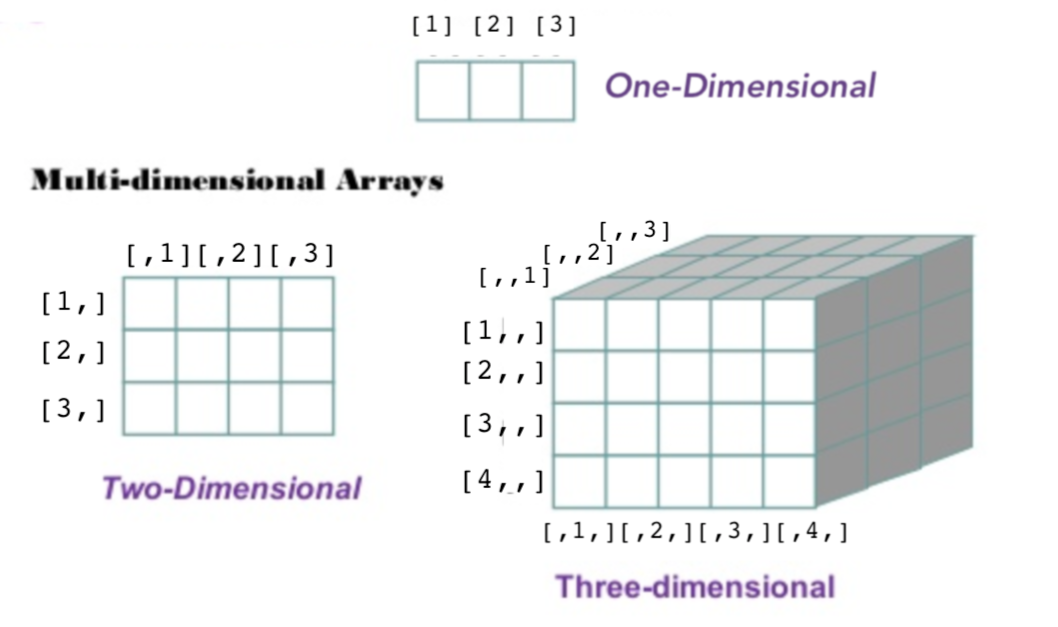
\includegraphics[height=0.72\textheight, width=0.8\textwidth]{arrays}
% \end{center}
% \end{frame}
% 
% 
% \begin{frame}[fragile]{Apply Functions (advanced)}
% <<size="scriptsize">>=
% (mm <- array(1:12, dim=c(3,4,2)))
% @
% \end{frame}
% 
% 
% \begin{frame}[fragile]{Apply Functions (advanced)}
% <<size="small">>=
% # results in a c(3,4,2)[c(1,2)] array
% apply(mm, c(1,2), sum)
% # results in a c(3,4,2)[c(3)] array
% apply(mm, 3, sum)
% @
% \end{frame}
% 
% 
% 
% \begin{frame}[fragile]{{\tt lapply}}
% \begin{itemize}
% \item The output of {\tt lapply} is a \emph{list}
% \item Unlike the generic {\tt apply} function which only takes \emph{arrays} as {\tt X} input, {\tt lapply} accepts lists and data frames for {\tt X}.
% \item The syntax looks is similar to {\tt apply()}
% $$\verb|lapply(X, FUN, ...)|$$
% where {\tt$\dots$} indicate the optional arguments of {\tt FUN()}
% \end{itemize}
% \end{frame}
% 
% 
% \begin{frame}[fragile]{{\tt lapply} function}
% \begin{itemize}
% \item  To see an advanced usage of {\tt lapply}, let's create a list of matrices.
% \item We will extract the third column from each of these matrices using the {\tt [} operator.
% \item To provide another example, we will also extract the second row of each.
% \end{itemize}
% \end{frame}
% 
% \begin{frame}[fragile]{{\tt lapply} function}
% <<size="scriptsize">>=
% mylist = list(matrix(1:12,nrow=2),matrix(1:12,nrow=3),matrix(1:12,nrow=4))
% mylist
% @
% \end{frame}
% 
% 
% 
% \begin{frame}[fragile]{{\tt lapply} function}
% <<>>=
% # extract the third column from each matrix in mylist
% (lcols = lapply(mylist,"[", , 3))
% # notice the row argument is left blank
% @
% Notice how the length of {\tt lcols} is equal to the length of {\tt mylist}.
% \end{frame}
% 
% % https://www.datacamp.com/community/tutorials/r-tutorial-apply-family#family good visual
% \begin{frame}[fragile]{{\tt lapply} function}
% <<>>=
% # extract the second row from each matrix in mylist
% (lrows = lapply(mylist,"[", 2, ))
% # notice the col argument is left blank
% @
% Notice how the length of {\tt lrows} is equal to the length of {\tt mylist}.
% \end{frame}
% 
% \begin{frame}[fragile]{{\tt lapply} function}\ref{lapplycell}
% We could have selected a single element, say the value in the first row and third column using the following code:
% <<>>=
% # extract the value in [1,3] for each matrix in mylist
% (crows = lapply(mylist,"[", 1, 3))
% @
% \end{frame}
% 
% 
% \begin{frame}{{\tt sapply()} function}
% \begin{itemize}
% \item The {\tt sapply()} function behaves like {\tt lapply()} but instead of returning a list, it attempts to convert the output to the most simple data structure possible.
% \item Consider the example we did on slide \ref{lapplycell}; the output was a list where each member was a single number.
% \item {\tt sapply} will coerce this output into a vector of length 3.
% \end{itemize}
% \end{frame}
% 
% 
% \begin{frame}[fragile]{{\tt sapply} function}
% We could have selected a single element, say the value in the first row and third column using the following code:
% <<>>=
% # extract the value in [1,3] for each matrix in mylist
% crows2 = sapply(mylist,"[", 1, 3)
% crows2
% @
% \end{frame}

% \begin{frame}[fragile]
% <<eval=TRUE, echo=FALSE>>=
% f <- '08RII.Rnw'
% knitr::purl(f)
% Stangle(f)
% @
% \end{frame}

% \begin{frame}[fragile]{}
% \end{frame}
% 
% \begin{frame}
% \begin{itemize}
% \item 
% \end{itemize}
% \end{frame}



\end{document}

